\section{Estado del arte}
\subsection{Búsquedas Scopus}
\begin{frame}
    \frametitle{Tendencia Scopus}
    \begin{columns}
      \column{0.5\textwidth}
      \begin{figure}
        \begin{center}
          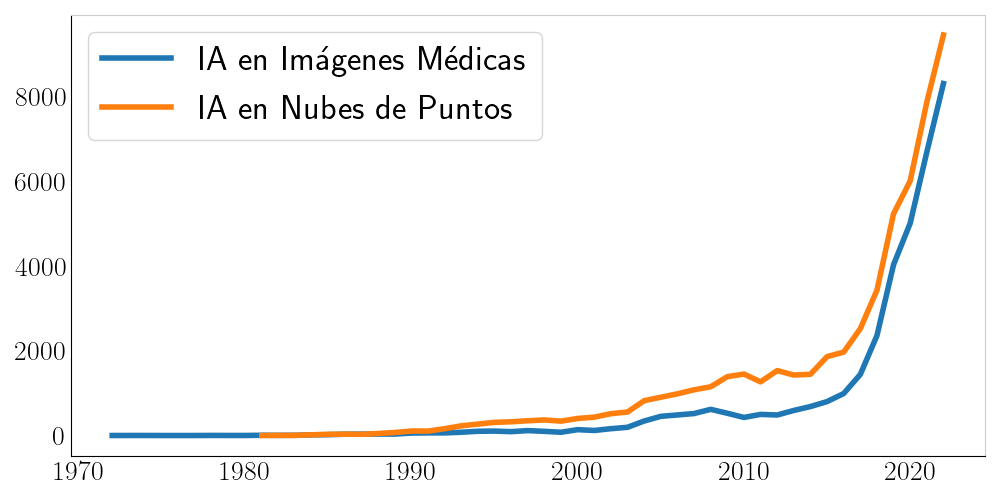
\includegraphics[width=\textwidth]{imagenes/chapter2/ScopusMLinMedicineAndPC}
        \end{center}
        \caption{Aprendizaje automático en medicina (azul) y nubes de puntos (naranja).
        \textbf{Ambos superan los 6000 documentos}.}
      \end{figure}
      
      \column{0.5\textwidth}
      \begin{figure}
        \begin{center}
          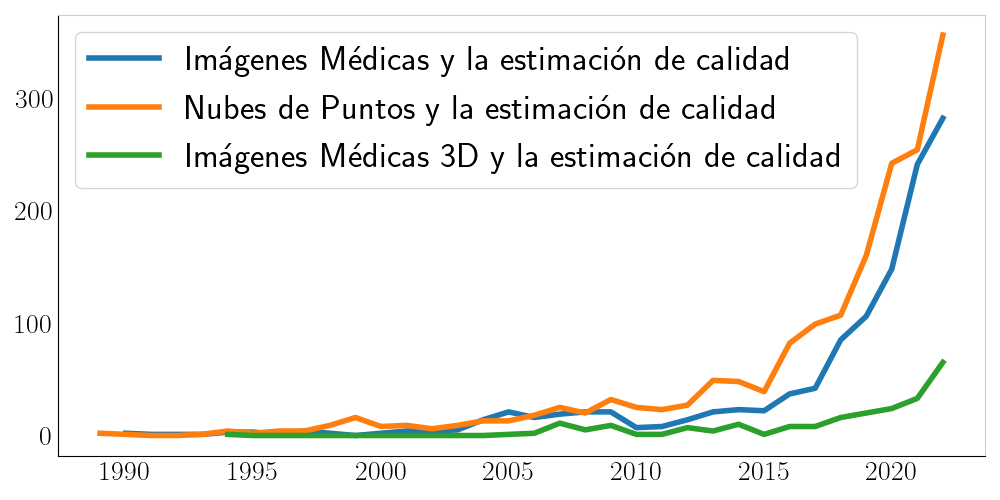
\includegraphics[width=\textwidth]{imagenes/chapter2/ScopusQualityAssessment}
        \end{center}
        \caption{Estimación de calidad en imágenes médicas (azul), nubes de puntos (naranja) 
          y en imágenes médicas 3D (verde). Esta última, tan solo llega a \textbf{62 publicaciones}}
      \end{figure}
    \end{columns}
\end{frame}

\note{
Como iba comentando anteriormente.
La estimación de calidad de imágenes y de objetos 3D, al ser un componente sumamente 
ligado al avance tecnológico y de las necesidades de manejo 
de información digital, 
ha tomado mayor interés en el comienzo del siglo actual.
Puede observarse en ambas Figuras que existe una tendencia creciente 
en relación a la aplicación de IA en las nubes de puntos y en imágenes médicas
Por otro lado, podemos afirmar lo mencionado sobre el bajo número de publicaciones 
en el ámbito biomédico y representaciones 3D, 
observando que, aunque hay también una tendencia positiva, en 2022 tenemos tan solo 60 publicaciones.
Esto se interpreta como un indicador de lo novedoso y pionero que es este proyecto.
}

\subsection{Estado del arte IQA: métricas}
\begin{frame}
  \frametitle{Estado del arte IQA: métricas}
  \begin{columns}
    \column{0.5\textwidth}
    \begin{enumerate}
      \item Están basados en los avances del conocimiento sobre el sistema visual humano (HVS):
        \begin{enumerate}
          \item Cuantificación de la señal. 
          \item La \textbf{sensibilidad al contraste}.
          \item Hipótesis de percepción a través de: \textbf{brillo, contraste y estructuras}.
          \item La \textbf{saliencia visual}. 
          \item Empleo de \textbf{modelos DL}.
        \end{enumerate}
    \end{enumerate}

    \column{0.5\textwidth}
  \begin{table}[htp]
    \footnotesize
    \centering
    \begin{tabular}{|c|c|c|c|}
      \hline
      \rowcolor[HTML]{FFC702}
      \cellcolor[HTML]{FFC702} &  \multicolumn{3}{c|}{\cellcolor[HTML]{FFC702}\textbf{LIVE}}\\ \cline{2-4}
      \rowcolor[HTML]{FFC702}
      \multirow{-2}{*}{\textbf{Métrica}} & SRCC & PLCC & RMSE \\ 
      \hline
                    \textbf<2>{PSNRHVS} & 0.919 & 0.903 & 12.540 \\
                    \hline
                     UQI & 0.894 & 0.899 & 11.982 \\
                    \hline
                     \textbf<3>{SSIM} & 0.948 & 0.845 & 8.946 \\
                    \hline
                     \textbf<4>{VSI} & 0.952 & 0.948 & 8.682 \\
                    \hline
                     \textbf<5>{WaDIQaM} & \textbf{0.970} & \textbf{0.980} & -\\ 
                    \hline 
    \end{tabular}
    \caption[Progreso de las métricas FR.]{
      Progreso de las métricas FR conforme avanza los conocimientos del HVS, ML y DL\footnotemark.
      }
      \label{tab:SOTAFRIQA}
  \end{table}
  \end{columns}
\footcitetext{SurveyOf2D3DMetrics}
\end{frame}

\note{
Para poner un poco de contexto, hablaremos del progreso de los métodos 2D de IQA, 
Con algunos ejemplos en la tabla a la derecha. Donde las 2 primeras 
columnas son coeficientes de correlación que deben acercarse a 1 y la última 
es la raíz del error que debe ser cercano a 0: 
Digamos que primeramente, surgieron métodos de cuantificación de señal como el primer ejemplo que vimos. 
A continuación empezaron a plasmarse conocimientos del sistema visual humano, utilizando 
por ejemplo nuestra sensibilidad al contraste. 
Seguidamente, propusieron la hipótesis de percepción a través de: brillo, contraste y
estructuras.
Con ello, surgió el famoso método de similitud estructural SSIM.
Los avances de dichos conocimientos supusieron incluso la codificación de la 
atención o saliencia visual humana con métodos como VSI. 
Y por último, siendo esta la tendencia actual, se empezaron a utilizar
métodos de extracción automática de características por 
medio de aprendizaje profundo.
}

\subsection{Estado del arte PCQA: métodos}
\begin{frame}
  \frametitle{Estado del arte PCQA: métodos}
  \begin{columns}
    \column{0.5\textwidth}
    \begin{enumerate}
      \item Métodos para casos específicos. 
      \item Extracción de características del vecindario del punto.
        \begin{enumerate}
          \item Características \textbf{geométricas}.
          \item Características \textbf{lumínicas}.
        \end{enumerate}
      \item Métodos genéricos por DL.
        \begin{enumerate}
          \item \textbf{Proyecciones 2D.}
          \item \textbf{Interpretación 3D directa.}
          \item Mixto.
        \end{enumerate}
    \end{enumerate}

    \column{0.5\textwidth}
      \begin{table}[htp]
          \footnotesize
          \centering
          \begin{tabular}{|c|c|c|c|c|}
              \hline
              \rowcolor[HTML]{FFC702}
              \cellcolor[HTML]{FFC702} & \multicolumn{2}{c|}{\cellcolor[HTML]{FFC702}\textbf{STJU-PCQA}} & \multicolumn{2}{c|}{\cellcolor[HTML]{FFC702}\textbf{WPC}} \\ 
              \cline{2-5}
             \multirow{-2}{*}{\cellcolor[HTML]{FFC702}\textbf{Método}}  &\multicolumn{1}{c|}{\cellcolor[HTML]{FFC702} PLCC} & \multicolumn{1}{c|}{\cellcolor[HTML]{FFC702}SRCC} & \multicolumn{1}{c|}{\cellcolor[HTML]{FFC702}PLCC} & \multicolumn{1}{c|}{\cellcolor[HTML]{FFC702}SRCC} \\
              \hline
              IT-PCQA & 0.58 & 0.63 & 0.55  & 0.54\\
              \hline
              \textbf<2->{NR3DQA} & 0.738 & 0.714 & 0.651 & 0.647\\
              \hline
              GPA-Net & 0.806 & 0.78 & - & - \\
              \hline
              ResSCNN & 0.86 & 0.81 & 0.72 & 0.75\\
              \hline
              \textbf<3->{VQA-PC} & 0.863 & 0.85 & 0.797 & 0.796\\
              \hline
              MM-PCQA & \textbf{0.92} & \textbf{0.91} & \textbf{0.83} & \textbf{0.83}\\
              \hline
          \end{tabular}
          \caption[Estado del arte de modelos NR-PCQA]{
          Resumen del estado del arte de modelos NR-PCQA en dos datasets SJTU y WPC.
        }
      \end{table}
  \end{columns}
\end{frame}

\note{
En el ámbito sin referencia, en particular las nubes de puntos, el avance es algo parecido. 
Primeramente parten de soluciones para distorsiones específicas, por ejemplo la compresión. 
A continuación, hacen uso de las estadísticas de escenas. En 3D esto consiste 
de la posibilidad de extraer características geométricas: como densidad de puntos
o lumínicas: como la consistencia del 
color. Estas características provienen del vecindario de un punto, y se extraen 
para todos los puntos. 
En concreto, un ejemplo de ello sería el modelo NR3DQA, del cual hablaremos más adelante.
No obstante, tanto en 3D como 2D,
más rápidamente pasan a utilizar métodos de aprendizaje profundo. 
En nubes de puntos se diferencian los siguientes métodos: los que proyectan dichas nubes 
a 2D para adaptar modelos IQA habituales y los que utilizan 
la representación 3D directamente. 
Recientemente incluso han surgido adaptaciones mixtas.
¿Pero.. qué es de las imágenes médicas?
}

\subsection{Estado del arte en imágenes médicas}
\begin{frame}
  \frametitle{Estado del arte en imágenes médicas}
  \begin{enumerate}
    \item \textbf{No existe} una imagen o representación \textbf{``sin distorsión''} en la medicina.
    \item Los métodos \textbf{actuales} utilizan adaptaciones \textbf{IQA} para 
      exámenes médicos concretos, como \textbf{MRI}.
    \item \textbf{No se ha encontrado} nada específico en la literatura sobre 
      métodos aplicados \textbf{directamente a 3D}.
      \begin{itemize}
        \item Reconstrucción.
        \item Escaneo láser forense.
        \item Segmentación.
      \end{itemize}
    \item Este TFG se centra en \textbf{la estimación de calidad, sin referencia, de nubes de puntos biomédicas}. 
  \end{enumerate}
  %\footcitetext{MRIVoxel}
\end{frame}

\note{
He aqui de explicar que las 62 publicaciones de las gráficas anteriores 
representan métodos que consisten de aproximaciones 2D, en particular para un 
tipo de examen concreto, por ejemplo resonancia magnética.
Resuelven el problema por medio de los múltiples planos anatómicos 2D generados 
por el mismo. 
Sin embargo, no se ha encontrado nada específico en la literatura para las 
reconstrucciones 3D generadas a partir de dichas imágenes médicas, por lo que es 
un campo sin explorar. 
No obstante, cada vez más se emplean 
volúmenes 3D en la medicina y, consecuentemente, es necesario explorar ese 
campo a pesar de la complejidad existente.
Es por ello, que este TFG se centra en la estimación de calidad, sin referencia, 
de nubes de puntos biomédicas.
}
